\chapter{Ergebnisse} % Speicher / Analyse / Zusammenfassung / Ergebnisse

Um den Speicher zu verstehen, klären wir vorab das Rückgabeformat der Speicherauszugs Befehle, sowie den Aufbau des Speichers der "`Jura Impressa S9"'.
Dieser Kaffeevollautomat besitzt einen \ac{RAM} für die Status, Messwerte und Zwischenberechnungen im Betrieb und einen \ac{EEPROM} für Einstellungen und Zählstände, die auch nach einer Stromunterbrechung erhalten bleiben.

\section{EEPROM}
Der \acf{EEPROM} umfasst 512 Bytes.
Über den Befehl \texttt{RT:<address>}, siehe Tabelle~\ref{tbl:kommandos}, lässt sich eine Zeile \ac{EEPROM} Speicher abfragen.
Die Adresse reicht von 0x00 bis 0xF0 in Sechzehner Sprüngen.
Als Antwort erhält man hinter dem kleingeschriebenen Kommando eine Zeichenkette bestehend aus 64 Hexadezimalzeichen.
Da immer zwei Hexadezimalzahlen ein Byte (8 Bit mit Werten von 0-255) repräsentieren umfasst eine \ac{EEPROM} Zeile 32 Bytes.
Über den Befehl \texttt{RE:<address>} können direkt Wörter im \ac{EEPROM} abgefragt werden. Die Adresse reicht von 0x00 bis 0xFF.
Die kleinste adressierbare Einheit, das Wort, besteht daher aus zwei Bytes, also vier Hexadezimalzeichen.

Im Folgenden wird vom "`Wort"', bzw. dessen ersten (XX) und zweiten (YY) Byte gesprochen.
Dabei gilt: "`Wort"' $= 256\times$"`erstes Byte"' $ + $ "`zweites Byte"' oder auch eine Antwort des Kaffeevollautomaten in der Form \texttt{re:YYXX}.

Abbildung~\ref{subfig:EEPROM} zeigt das Speicherschema des \ac{EEPROM}.

\begin{sidewaysfigure}
    \centering%
    \fboxsep=0.02\textwidth%
    \subfigure[EEPROM]{\label{subfig:EEPROM}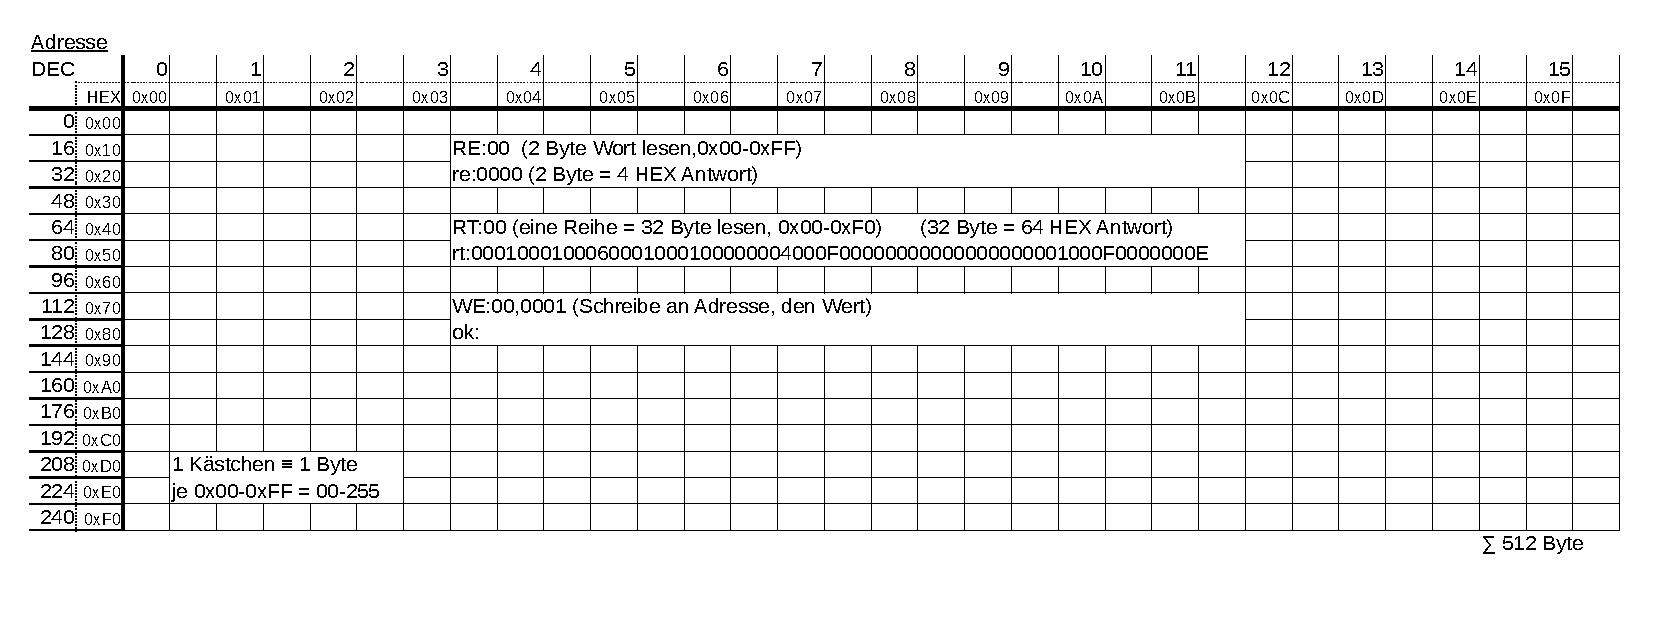
\includegraphics[scale=0.7,trim={0 1.1cm 0 0},clip]{images/chapter_5/Speicher-Schema-Jura-EEPROM}}\\%
    \subfigure[RAM]{\label{subfig:RAM}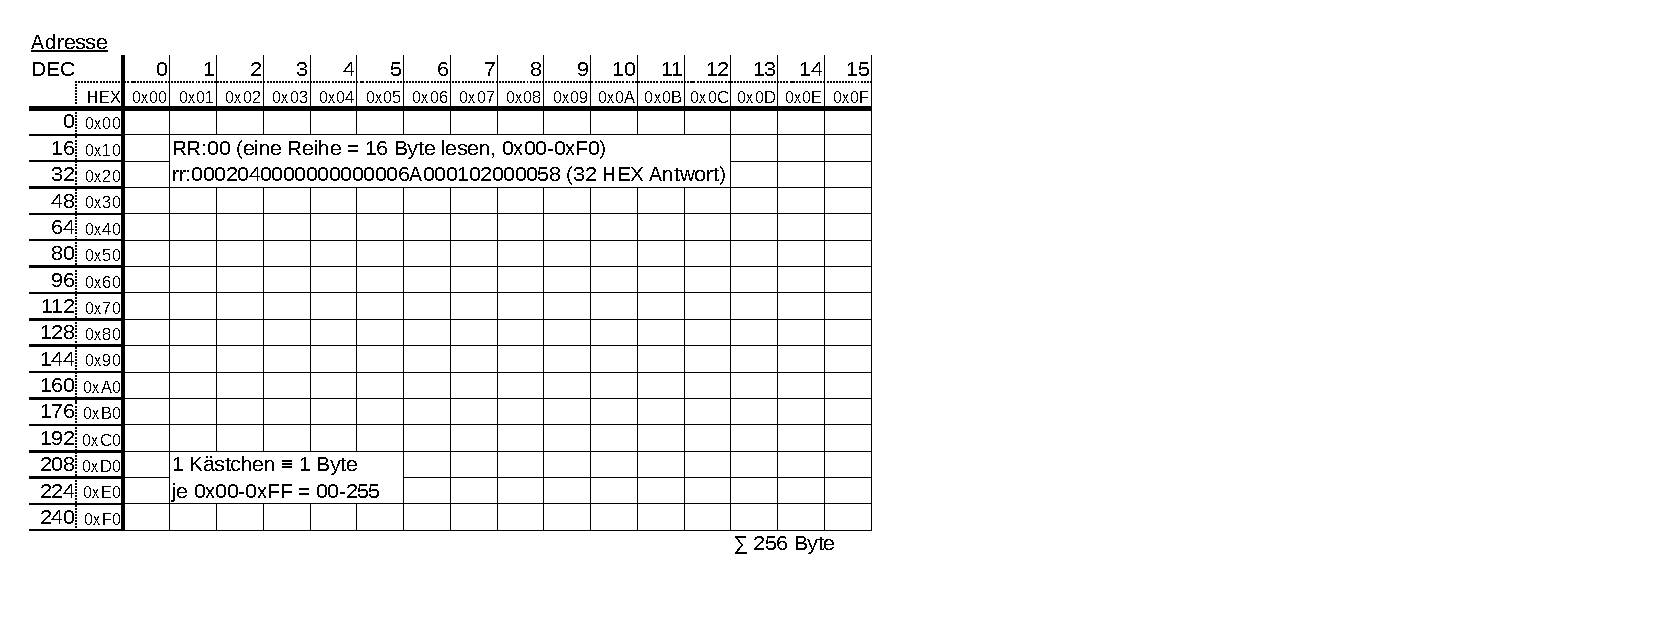
\includegraphics[scale=0.7,trim={0 1.1cm 0 0},clip]{images/chapter_5/Speicher-Schema-Jura-RAM}}%
    \caption{Speicherschema der Jura Impressa S9}
    \label{fig:Speicherschema}
\end{sidewaysfigure}

\subsection{Kaffeezubereitung}\label{subsec:ErgebnisKaffeezubereitung}
Der Kaffeevollautomat unterscheidet bei der Zubereitung zwischen einem einmaligen Pulver-Kaffee und der normalen Zubereitung über das Bohnenfach.
Nur im Falle eines \bezeichnung{Pulver-Kaffees} zählt die Maschine den Zähler in Wort \wort{06} um einen hoch.
\bezeichnung{1 großer Kaffee}, \bezeichnung{2 große Kaffees}, \bezeichnung{1 kleiner Kaffee}, \bezeichnung{2 kleine Kaffees} und ein \bezeichnung{Spezialkaffee} werden bei einer Zubereitung über das Bohnenfach einzeln in den Zählern der Wörter \wort{00} bis \wort{04} in eben dieser Reihenfolge erfasst.
Der in den Einstellungen des Kaffeevollautomaten angezeigte \bezeichnung{Bezüge Zähler} gibt die Summe der bis hier genannten \wert{sechs Zähler} aus.

Die Zähler in den Worten \wort{0F} und \wort{15} werden bei \bezeichnung{jeder Zubereitung} jeweils um \wert{einen inkrementiert}, egal ob ein einfacher oder ein doppelter Bezug erfolgt, ebenso egal ob als Pulver-Kaffee oder über das Bohnenfach.
Erreicht der Wert in \wort{0F} eine Anzahl von \wert{220} Bezügen erscheint eine Reinigungsankündigung.

Darüber hinaus gibt es zwei \bezeichnung{partielle Zähler} in den Worten \wort{0D} und \wort{10}, die ungefähr bei jeder dritten Zubereitung oder Spülung um \wert{einen inkrementiert} werden.
Der genaue Grund dafür ist bisher unbekannt.

Der \bezeichnung{Trester} Stand in der Schale dieses Kaffeevollautomaten wird nicht gemessen, sondern bei jeder Zubereitung in \bezeichnung{zwei Zählern} vermerkt.
In Wort \wort{0E} ist nicht genau bekannt, wann um einen inkrementiert wird.
Ab einem Wert von \wert{16} folgt dann aber die Meldung "`Trester leeren"'.\\
Ein zweiter Trester Zähler befindet sich hinter Wort \wort{34}.
Je nach eingestellter Pulvermenge wird der Zähler um mehrere Einheiten erhöht.
Ab einem Wert von \wert{960} folgt ebenfalls die Meldung "`Trester leeren"'.\\
Beide Werte werden bei der Entnahme der Schale für mindestens 8 Sekunden automatisch auf \wert{0} zurück gesetzt.
Dies geschieht auch bei einer Reinigung.

\subsection{Kaffee Einstellungen}
Die \bezeichnung{Pulvermenge} kann in 29 Stufen auf einer Skala von \wert{0} bis \wert{28}, für einen kleinen Kaffee in Wort \wort{82}, für einen großen Kaffee in Wort \wort{83} und für einen Spezialkaffee in Wort \wort{84}, jeweils im zweiten Byte eingestellt werden.
Der Standardwert, über die \texttt{[N]}-Taste am Kaffeevollautomaten, beträgt \wert{5} für einen kleinen Kaffee, \wert{8} für einen großen Kaffee und \wert{11} für einen Spezialkaffee.
Die Menge wird automatisch für zwei kleine Kaffees und zwei große Kaffees hochgerechnet.

Die \bezeichnung{Wassermenge} eines kleinen Kaffees wird in Wort \wort{86}, eines großen Kaffees in Wort \wort{87} und eines Spezialkaffees in Wort \wort{88} über beide Bytes hinweg gespeichert.
Der Standardwert, über die \texttt{[N]}-Taste am Kaffeevollautomaten, beträgt \wert{180} für einen kleinen Kaffee, \wert{340} für einen großen Kaffee und \wert{380} für einen Spezialkaffee.
Auch hier wird die Menge automatisch auf zwei kleine Kaffees und zwei große Kaffees hochgerechnet.

Die \bezeichnung{Temperatur} kann für einen kleinen Kaffee, für einen großen Kaffee und für einen Spezialkaffee jeweils normal oder hoch eingestellt werden.
Der Standardwert liegt bei \wert{0} im zweiten Byte von Wort \wort{85} und bedeutet eine normale Temperatur für alle Sorten.
Möchte man einen kleinen Kaffee auf heiß stellen addiert man \wert{1}, für einen großen Kaffee addiert man \wert{2} und für einen Spezialkaffee addiert man \wert{4} auf den alten Wert.
Der Wert \wert{7} ist somit das Maximum und bedeutet eine heiße Temperatur für alle Sorten.

\subsection{(Tee-) Wasser- und Dampfportionen}
In Wort \wort{BB} wird die Größe einer \bezeichnung{Dampfportion} in Sekunden abgespeichert.
Nach der eingestellten Zeit endet automatisch die Dampfausgabe am Kaffeevollautomaten beim Bezug einer Dampfportion.

In Wort \wort{BC} wird die Größe einer \bezeichnung{Teeportion} abgespeichert.
Die Einheit ist hier nicht bekannte, es könnte sich aber um die Größenordnung von $0,1$ Sekunden handeln.
Wird das Drehrad von der Position "`Kaffeetasse"' auf "`Teeauslass"' gestellt wird eine Teeportion an heißem Wasser ausgegeben und automatisch beendet.

\subsection{Weitere Maschinen Einstellungen}
Wort \wort{24} speichert im ersten Byte die Information der \bezeichnung{Wasserhärte}.
Der Wert \wert{0} deaktiviert die Wasserhärte-Funktion.
Die Werte \wert{1} bis \wert{4} repräsentieren die vier Stufen, die im Benutzerhandbuch zur Maschine ausgeführt werden.
In dem zweiten Byte wird der \bezeichnung{Economy Mode} gesteuert.
\wert{1} aktiviert diesen und \wert{0} deaktiviert diesen.

In Wort \wort{25} wird die \bezeichnung{automatische Einschaltzeit} des Kaffeevollautomaten bei eingestellter Uhrzeit gespeichert.
Das erste Byte speichert die \bezeichnung{Stunde} in einem Wertebereich von \wert{0} bis \wert{23} und das zweite Byte die \bezeichnung{Minute} in einem Wertebereich von \wert{0} bis \wert{59}.
Der deaktivierte Zustand ist gegeben, wenn die Stunde auf \wert{0} und die Minute auf \wert{128} steht.

In Wort \wort{26} steht im zweiten Byte die \bezeichnung{automatische Ausschaltzeit}.
Möglich sind die Werte \wert{0}, \wert{1}, \wert{2}, \wert{4}, \wert{6}, \wert{8}, \wert{10}, \wert{12}, \wert{14}, \wert{16} und \wert{18}.
Wert \wert{0} bedeutet deaktiviert, die übrigen Werte geben ein Intervall in halben Stunden an, nach dem sich der Kaffeevollautomat automatisch abschaltet.
Das bedeutet, dass $0,5$ Stunden das Minimum und $9$ Stunden das Maximum ist.

In Wort \wort{31} befindet sich nach \cite{GitCoffeeMachine} der \bezeichnung{Maschinen Typ}.
Dieser kann mittels \texttt{RE:31} gelesen und mittels \texttt{WE:31,xxxx} überschrieben werden.

In Wort \wort{7D} befindet sich ein Zähler, der bei jedem Einschaltvorgang inkrementiert wird und somit die totale \bezeichnung{Anzahl an Einschaltvorgängen} erfasst.
Ausschaltvorgänge werden nicht vermerkt.

In Wort \wort{81} befindet sich im zweiten Byte die \bezeichnung{Spracheinstellung}.
Die folgenden Werte repräsentieren folgende Sprachen:
\wert{0} Deutsch,
\wert{16} Italienisch,
\wert{32} Niederländisch, 
\wert{48} Spanisch,
\wert{64} Englisch,
\wert{80} Französisch und
\wert{96} Portugiesisch.

In Wort \wort{B0} wird im zweiten Byte mit einem Wert von \wert{16} der \bezeichnung{Inkasso Modus} aktiviert und mit einem Wert von \wert{0} deaktiviert.
Bei eingeschaltetem Inkasso Modus erfolgt kein Bezug mehr über die Bezugstasten an der Vorderseite des Gehäuses, jedoch wird die gedrückte Taste über die \ac{UART} Schnittstelle weitergeleitet.
Mit dem entsprechenden Befehl kann über die serielle Schnittstelle dann aber die Zubereitung angestoßen werden.\\
Man erhält von dem Kaffeevollautomaten auf Knopfdruck
\texttt{?PAE} für einen kleinen Kaffe,
\texttt{?PAF} für zwei kleine Kaffees,
\texttt{?PAA} für einen großen Kaffee,
\texttt{?PAB} für zwei große Kaffees,
\texttt{?PAG} für einen Spezialkaffee,
\texttt{?PAJ} für eine Dampfportion,
\texttt{?PAI} für Wasserdampf und
\texttt{?PAK} für heißes Teewasser.

\subsection{Filter}
In Wort \wort{7D} wird im zweiten Byte gespeichert, ob ein \bezeichnung{Filter eingelegt} ist.
Der Wert \wert{0} steht für "`nein"', \wert{8} bedeutet "`ja"'.
Dieser Wert hat Einfluss auf Zähler an anderen Speicherstellen, die zum Teil nur im Falle eines "`ja"' weiter gezählt werden.

In Wort \wort{05} befindet sich ein \bezeichnung{Filter-Zähler}, der für jeden neu eingesetzten Filter inkrementiert wird.

Bei einem Filterwechsel werden die Werte in den Worten \wort{B1}, \wort{B3} und \wort{C1} (Bedeutung unbekannt) auf \wert{0} zurück gesetzt.
Erreicht der Wert in Wort \wort{B3} einen Stand von \wert{500} sind 50 Liter Wasserdurchfluss erreicht und der Filter muss gewechselt werden.
Laut Handbuch sollte ebenso spätestens nach zwei Monaten der Filter gewechselt werden.

\subsection{Spülung}
In Wort \wort{07} befindet sich ein Gesamtzähler für die \bezeichnung{Anzahl an Spülungen}.

Die partiellen Zähler hinter den Worten \wort{0D} und \wort{10} werden auch bei einer Spülung angestoßen.
Der Wert in den Worten \wort{11}, bei eingelegtem Filter auch \wort{B1} und \wort{B3}, werden bei einer Spülung um \wert{1} inkrementiert.
Erreicht der Wert in Wort \wort{B3} den Wert \wert{500} sind 50 Liter Wasserdurchfluss erreicht und der Filter muss gewechselt werden.

\subsection{Reinigung}
Die Meldung wird ausgelöst, wenn der Wert in Wort \wort{0F} einen Wert von \wert{220} erreicht hat oder der Wert in Wort \wort{11} einen Wert von \wert{180} erreicht hat.
Im ersten Fall sind 220 Bezüge erfolgt, im zweiten Fall waren es 180 Spülungen.

In den Worten \wort{07} (Anzahl an Spülungen), \wort{08} (Bedeutung unbekannt), \wort{7C} (Bedeutung unbekannt) und am Ende nach der abschließenden Spülung bei eingelegtem Filter in \wort{B1} und \wort{B3} wird der Wert um \wert{1} inkrementiert.
In den Worten \wort{10} und \wort{B3} wird der Wert um \wert{10} inkrementiert.
Die Werte in den Worten \wort{0E}, \wort{0F}, \wort{11} und \wort{34} werden zurück auf \wert{0} gesetzt.
Wort \wort{11} wird jedoch anschließend an die abschließende Spülung gleich wider um \wert{1} inkrementiert.

Wort \wort{29} Byte eins wird zu Beginn einer Reinigung auf \wert{65} gesetzt und am Ende auf \wert{0} zurück gesetzt.

\section{RAM}\label{sec:ErgebnisseRAM}
Der \acf{RAM} umfasst 256 Bytes.
Der Lesebefehl für eine \ac{RAM} Zeile lautet: \texttt{RR:<address>}.
Die Adresse reicht hier von 0x00 bis 0xFF, sodass hier die kleinste Einheit ein Byte, bestehend aus zwei Hexadezimalzeichen, ist.
Jedes Byte besitzt acht Bits, die im Folgenden mit den Nummern 0 ($=1\times 2^0$) bis 7 ($=1\times 2^7$) bezeichnet werden.\\
Abbildung~\ref{subfig:RAM} zeigt das Speicherschema des \ac{RAM}.

Aufgrund starker, aber zum Teil regelmäßiger Schwankungen, wurden die folgenden Bytes über mehrere Speicherauszüge ohne zwischenzeitliche Veränderungen ermittelt und \bezeichnung{für diese Arbeit ausgeblendet}:
\wort{02}, \wort{09}, \wort{0C}, \wort{1C} bis \wort{21}, \wort{27}, \wort{28}, \wort{2A}, \wort{2C}, \wort{2E}, \wort{41}, \wort{66}, \wort{67}, \wort{6A}, \wort{6C}, \wort{70}, \wort{7C}, \wort{94}, \wort{95}, \wort{97}, \wort{9C}, \wort{9D}, \wort{A2}, \wort{F1} und \wort{FC} bis \wort{FF}.

Die Aufschlüsselung und der Bezugspunkt für die im Folgenden genannten Rubriken sind die Spalten der Tabelle~\ref{tbl:RAM1} und der Tabelle~\ref{tbl:RAM2}.

Unterstrichene und hervorgehobene Zellen sind "`immer"' abfragbar.
Die einzige Voraussetzung ist die in Abschnitt \ref{subsec:AufbauUndVerkabelung} beschriebene Verkabelung, sowie eine angelegte Netzspannung an den Kaffeevollautomaten.
Der Kaffeevollautomat \underline{muss} sich dann \underline{nicht} im eingeschalteten Zustand befinden.

Eingeklammerte Zellen haben sind nicht exklusiv für die genannte Rubrik, sie teilen sich den Wert mit weiteren Funktionen.

\begin{sidewaystable}
  \footnotesize\centering
  \begin{tabular}[htp]{llllllllll}
  \THc{1}{l}{Funktion} &
  \THc{1}{c}{\rotatebox{50}{Maschine an}} &
  \THc{1}{c}{\rotatebox{50}{Schale fehlt}} &
  \THc{1}{c}{\rotatebox{50}{Schale leeren}} &
  \THc{1}{c}{\rotatebox{50}{Trester leeren}} &
  \THc{1}{c}{\rotatebox{50}{Wasser füllen}} &
  \THc{1}{c}{\rotatebox{50}{Gerät reinigen}} &
  \THc{1}{c}{\rotatebox{50}{Maschine spült}} &
  \THc{1}{c}{\rotatebox{50}{Abschließend spülen}} &
  \THc{1}{c}{\rotatebox{50}{Tassenbeleuchtung}} \\

%
  \TRhc{1}{l}{\textbf{Byte}} &
  \TRhc{1}{l}{\wort{03}} &
  \TRhc{1}{l}{\wort{0E}} &
  \TRhc{1}{l}{\wort{04}} &
  \TRhc{1}{l}{\wort{04}} &
  \TRhc{1}{l}{\wort{04}} &
  \TRhc{1}{l}{\wort{10}} &
  \TRhc{1}{l}{\wort{03}} &
  \TRhc{1}{l}{\wort{0D}} &
  \TRhc{1}{l}{\wort{0F}} \\
  
  Bit &
  \immer{\bitTrue{2}} &
  \immer{\bitTrue{2}} &
  \geteilt{\bitTrue{3}} &
  \bitTrue{5} &
  \geteilt{\bitTrue{3}} &
  \bitTrue{7} &
  \geteilt{\bitTrue{6,3,1}} &
  \bitTrue{3 oder 2} &
  \bitTrue{2 oder 1} \\
  
  \belowbodyrule
%
  \TRhc{1}{l}{\textbf{Byte}} &
  \TRhc{1}{l}{\wort{05}} &
  \TRhc{1}{l}{\wort{16}} &
  \TRhc{1}{l}{\wort{0E}} &
  \TRhc{1}{l}{\wort{0E}} &
  \TRhc{1}{l}{\wort{0E}} &
  \TRhc{1}{l}{\wort{22}} &
  \TRhc{1}{l}{\wort{13}} &
  \TRhc{1}{l}{} &
  \TRhc{1}{l}{} \\
  
  Bit &
  \immer{\bitTrue{5}} &
  \bitFalse{0} &
  \immer{\bitTrue{4}} &
  \bitTrue{5} &
  \immer{\bitTrue{6}} &
  \bitTrue{4} &
  \bitTrue{3,1} &
   &
   \\
  
  \belowbodyrule
%
  \TRhc{1}{l}{\textbf{Byte}} &
  \TRhc{1}{l}{\wort{16}} &
  \TRhc{1}{l}{\wort{29}} &
  \TRhc{1}{l}{\wort{1B}} &
  \TRhc{1}{l}{\wort{80}} &
  \TRhc{1}{l}{\wort{0F}} &
  \TRhc{1}{l}{} &
  \TRhc{1}{l}{\wort{17}} &
  \TRhc{1}{l}{} &
  \TRhc{1}{l}{} \\
  
  Bit &
  \immer{\bitTrue{1}} &
  \immer{\bitFalse{2}} &
  \immer{\bitTrue{1}} &
  \immer{\bitTrue{1,0}} &
  \immer{\bitFalse{4}} &
   &
  \bitTrue{1} &
   &
   \\
  
  \belowbodyrule
%
  \TRhc{1}{l}{\textbf{Byte}} &
  \TRhc{1}{l}{\wort{44}} &
  \TRhc{1}{l}{\wort{69}} &
  \TRhc{1}{l}{\wort{29}} &
  \TRhc{1}{l}{} &
  \TRhc{1}{l}{\wort{4C}} &
  \TRhc{1}{l}{} &
  \TRhc{1}{l}{\wort{62}} &
  \TRhc{1}{l}{} &
  \TRhc{1}{l}{} \\
  
  Bit &
  \immer{\bitTrue{0}} &
  \bitFalse{0} &
  \immer{\bitTrue{6-3}} &
   &
  \geteilt{\bitFalse{0}} &
   &
  \geteilt{\bitTrue{1}} &
   &
   \\
  
  \belowbodyrule
%
  \TRhc{1}{l}{\textbf{Byte}} &
  \TRhc{1}{l}{} &
  \TRhc{1}{l}{} &
  \TRhc{1}{l}{\wort{2B}} &
  \TRhc{1}{l}{} &
  \TRhc{1}{l}{\wort{91}} &
  \TRhc{1}{l}{} &
  \TRhc{1}{l}{} &
  \TRhc{1}{l}{} &
  \TRhc{1}{l}{} \\
  
  Bit &
   &
   &
  \immer{\bitTrue{6-3}} &
   &
  \geteilt{\bitFalse{1}} &
   &
   &
   &
   \\
  
  \belowbodyrule
%
  \TRhc{1}{l}{\textbf{Byte}} &
  \TRhc{1}{l}{\wort{1A}} &
  \TRhc{1}{l}{} &
  \TRhc{1}{l}{} &
  \TRhc{1}{l}{} &
  \TRhc{1}{l}{} &
  \TRhc{1}{l}{} &
  \TRhc{1}{l}{\wort{68}} &
  \TRhc{1}{l}{} &
  \TRhc{1}{l}{} \\
  
  Bit &
  \immer{\bitFalse{2}} &
   &
   &
   &
   &
   &
  \geteilt{\bitTrue{6}} &
   &
   \\
  
  Bit &
  \immer{\bitTrue{1,0}} &
   &
   &
   &
   &
   &
  \geteilt{\bitFalse{5,4}} &
   &
   \\
  \belowbodyrule
  \end{tabular}
  \caption{Speicherpositionen im \ac{RAM} (1)}
  \label{tbl:RAM1}
\end{sidewaystable}
\begin{sidewaystable}
  \footnotesize\centering
  \begin{tabular}[htp]{lllllllllll}
  \THc{1}{l}{Funktion} &
  \THc{1}{c}{\rotatebox{50}{Filter wechseln}} &
  \THc{1}{c}{\rotatebox{50}{Hahn offen}} &
  \THc{1}{c}{\rotatebox{50}{Teeportion}} &
  \THc{1}{c}{\rotatebox{50}{Dampfbezug}} &
  \THc{1}{c}{\rotatebox{50}{Wasserdampfportion}} &
  \THc{1}{c}{\rotatebox{50}{Pulver füllen}} &
  \THc{1}{c}{\rotatebox{50}{Bohnen füllen}} &
  \THc{3}{c}{\rotatebox{50}{Zubereitung}} \\
  
  \THsub{1}{l}{} &
  \THsub{1}{l}{} &
  \THsub{1}{l}{} &
  \THsub{1}{l}{} &
  \THsub{1}{l}{} &
  \THsub{1}{l}{} &
  \THsub{1}{l}{} &
  \THsub{1}{l}{} &
  \THsub{1}{c}{immer} &
  \THsub{1}{c}{1. Schritt} &
  \THsub{1}{c}{2. Schritt} \\

%
  \TRhc{1}{l}{\textbf{Byte}} &
  \TRhc{1}{l}{\wort{10}} &
  \TRhc{1}{l}{\wort{04}} &
  \TRhc{1}{l}{\wort{03}} &
  \TRhc{1}{l}{\wort{04}} &
  \TRhc{1}{l}{\wort{03}} &
  \TRhc{1}{l}{\wort{04}} &
  \TRhc{1}{l}{\wort{0E}} &
  \TRhc{1}{l}{} &
  \TRhc{1}{l}{} &
  \TRhc{1}{l}{\wort{03}} \\
  
  Bit &
  \bitTrue{5} &
  \geteilt{\bitTrue{3}} &
  \geteilt{\bitTrue{6}} &
  \geteilt{\bitTrue{3}} &
  \geteilt{\bitTrue{3}} &
  \bitTrue{0} &
  \bitTrue{7} &
   &
   &
  \bitTrue{1} \\
  
  \belowbodyrule
%
  \TRhc{1}{l}{\textbf{Byte}} &
  \TRhc{1}{l}{\wort{22}} &
  \TRhc{1}{l}{\wort{0F}} &
  \TRhc{1}{l}{\wort{0B}} &
  \TRhc{1}{l}{\wort{0B}} &
  \TRhc{1}{l}{\wort{0B}} &
  \TRhc{1}{l}{} &
  \TRhc{1}{l}{} &
  \TRhc{1}{l}{} &
  \TRhc{1}{l}{} &
  \TRhc{1}{l}{\wort{0B}} \\
  
  Bit &
  \bitTrue{3} &
  \immer{\bitFalse{6}} &
  \geteilt{\bitFalse{3}} &
  \geteilt{\bitFalse{3}} &
  \geteilt{\bitFalse{3}} &
   &
   &
   &
   &
  \geteilt{\bitFalse{3}} \\
    
  \belowbodyrule
%
  \TRhc{1}{l}{\textbf{Byte}} &
  \TRhc{1}{l}{\wort{F8}} &
  \TRhc{1}{l}{\wort{4C}} &
  \TRhc{1}{l}{\wort{0F}} &
  \TRhc{1}{l}{\wort{13}} &
  \TRhc{1}{l}{\wort{13}} &
  \TRhc{1}{l}{} &
  \TRhc{1}{l}{} &
  \TRhc{1}{l}{} &
  \TRhc{1}{l}{} &
  \TRhc{1}{l}{\wort{17}} \\
  
  Bit &
  \immer{\bitTrue{0}} &
  \geteilt{\bitFalse{0}} &
  \immer{\bitTrue{5}} &
  \bitTrue{2-0} &
  \bitTrue{2,0} &
   &
   &
   &
   &
  \bitTrue{3} \\
  
  \belowbodyrule
%
  \TRhc{1}{l}{\textbf{Byte}} &
  \TRhc{1}{l}{} &
  \TRhc{1}{l}{\wort{4D}} &
  \TRhc{1}{l}{\wort{4C}} &
  \TRhc{1}{l}{\wort{49}} &
  \TRhc{1}{l}{\wort{49}} &
  \TRhc{1}{l}{} &
  \TRhc{1}{l}{} &
  \TRhc{1}{l}{} &
  \TRhc{1}{l}{} &
  \TRhc{1}{l}{\wort{62}} \\
  
  Bit &
   &
  \bitTrue{3,1} &
  \geteilt{\bitFalse{0}} &
  \geteilt{\bitTrue{0}} &
  \geteilt{\bitTrue{0}} &
   &
   &
   &
   &
  \geteilt{\bitTrue{1}} \\
  
  \belowbodyrule
%
  \TRhc{1}{l}{\textbf{Byte}} &
  \TRhc{1}{l}{} &
  \TRhc{1}{l}{} &
  \TRhc{1}{l}{\wort{68}} &
  \TRhc{1}{l}{\wort{4C}} &
  \TRhc{1}{l}{\wort{4C}} &
  \TRhc{1}{l}{} &
  \TRhc{1}{l}{} &
  \TRhc{1}{l}{} &
  \TRhc{1}{l}{} &
  \TRhc{1}{l}{\wort{68}} \\
  
  Bit &
   &
   &
  \geteilt{\bitTrue{6}} &
  \geteilt{\bitFalse{0}} &
  \geteilt{\bitFalse{0}} &
   &
   &
   &
   &
  \geteilt{\bitFalse{5}} \\
  
  \belowbodyrule
%
  \TRhc{1}{l}{\textbf{Byte}} &
  \TRhc{1}{l}{\wort{F9}} &
  \TRhc{1}{l}{} &
  \TRhc{1}{l}{\wort{4D}} &
  \TRhc{1}{l}{} &
  \TRhc{1}{l}{} &
  \TRhc{1}{l}{} &
  \TRhc{1}{l}{} &
  \TRhc{1}{l}{\wort{0A}} &
  \TRhc{1}{l}{\wort{03}} &
  \TRhc{1}{l}{} \\
  
  Bit &
  \bitTrue{7,6,5,4,2} &
   &
  \bitFalse{3,1} &
   &
   &
   &
   &
  \bitTrue{6} &
  \bitTrue{7,4} &
   \\
  
   &
  (\wert{$0_{10} \rightarrow 244_{10}$}) &
   &
  \bitTrue{0} &
   &
   &
   &
   &
  (2-0: "`Kaffee"') &
  (7 nicht manuell) &
   \\
  \belowbodyrule
  \end{tabular}
  \caption{Speicherpositionen im \ac{RAM} (2)}
  \label{tbl:RAM2}
\end{sidewaystable}

\subsection{Maschine an}
Sobald der Kaffeevollautomat eingeschaltet wird ändern sich die Werte mehrerer Speicherstellen im \ac{RAM}.
Tabelle~\ref{tbl:RAM1} zeigt die regelmäßigen Änderungen beim Einschalten in der ersten Spalte "`Maschine an"'.
Der Umschwung der sieben Bits erfolgt sofort nach der Betätigung des "`Ein"'-Schalters, selbst wenn sich der Kaffeevollautomat noch aufwärmt und "`Bitte warten"' anzeigt.
Eine Änderung nach der Aufwärmphase konnte nicht festgestellt werden.

Beim Ausschaltet geschehen die Änderungen vice versa.

\subsection{Schale fehlt}
Die beiden linken Kontakte, die eine eingesetzte Schale verbindet, sind voneinander getrennt.
Ohne eine eingesetzte Schale schaltet der Kaffeevollautomat sicherheitshalber alle Tätigkeiten ab.
Dies wird auch im ausgeschalteten Zustand vermerkt.

Die Änderungen sind in Tabelle~\ref{tbl:RAM1} in der zweiten Spalte dargestellt.
In \bytebit{16}{0} und in \bytebit{69}{0} steht nur eine \wert{0}, wenn der Kaffeevollautomat eingeschaltet ist.
Die an anderen beiden Bits enthalten zu jeder Zeit den aktuellen Status.

\subsection{Schale leeren}
Die linken beiden und der rechte Kontakt sind kurzgeschlossen.
Der Wasserstand in der Auffangschale ist dann gefährlich hoch und der Kaffeevollautomat schaltet sicherheitshalber alle Tätigkeiten ab.
Dies wird auch im ausgeschalteten Zustand vermerkt.

Die Änderungen sind in Tabelle~\ref{tbl:RAM1} in der dritten Spalte dargestellt.

\subsection{Trester leeren}
Hat einer der beiden Trester Zähler seine Grenze erreicht, erfolgt die Aufforderung den Trester zu leeren.
Indem die Schale für mindestens acht Sekunden entnommen wird, werden beide Zähler auf \wert{0} zurück gesetzt.

Eine wichtige Ergänzung zur Tabelle~\ref{tbl:RAM1} ist, dass nur der Trester Zähler im \ac{EEPROM} in Wort \wort{34} die Änderung im \ac{RAM} in \bytebits{80}{1}{0} auslöst.
Um allgemein diese Meldung ausschließen zu können muss sich der Kaffeevollautomat im eingeschalteten Zustand befinden.

\subsection{Wasser füllen} % Wassertank entnommen
Bei dieser Meldung schließt der magnetische Schwimmer im Wassertank nicht den Kontakt und die Meldung leuchtet auf.
Der Wasserspiegel kann hierbei zu niedrig sein oder der Wassertank wurde zum Auffüllen oder Wasser Wechseln entnommen.
Dies wird auch im ausgeschalteten Zustand vermerkt.

Die Änderungen sind in Tabelle~\ref{tbl:RAM1} in der fünften Spalte dargestellt.

\subsection{Gerät reinigen}
Sind 220 Bezüge oder 180 Spülungen erreicht, wird eine Reinigung gefordert.
In \bytebit{10}{7} und in \bytebit{22}{4} steht dann je eine \wert{1}, siehe Tabelle~\ref{tbl:RAM1} Spalte sechs.

\subsection{Maschine spült}
Wenn der Kaffeevollautomat eine Spülung vornimmt wird dies in mehreren Bits vermerkt.
Die Änderungen sind in Tabelle~\ref{tbl:RAM1} in der siebten Spalte dargestellt.

\subsection{Maschine vor dem Ausschalten spülen}
Der Kaffeevollautomat erzwingt eine Spülung vor dem Ausschalten, wenn während der Betriebszeit ein Kaffeebezug erfolgte, ohne eine abschließende Spülung vorgenommen zu haben.
In \bytebits{0D}{3}{2} steht in diesem Fall mal an dem einen und mal an dem anderen Bit eine \wert{1}.
Dieser Merker befindet sich sehr wahrscheinlich hier, auch wenn die genau Bedeutung der einzelnen Bits nicht sicher bekannt ist.

\subsection{Tassenbeleuchtung}
Bei einer Zubereitung oder laut Benutzerhandbuch auch durch das Drücken einer beliebigen Taste im ausgeschalteten Zustand wird die Tassenbeleuchtung eingeschaltet.
Nach drei Minuten schaltet die Tassenbeleuchtung dann wieder automatisch ab.

In \bytebitss{0F}{2}{1} steht bei eingeschalteter Tassenbeleuchtung "`immer"' mindestens eine \wert{1}.
Beim Betreten des Menüs oder auch beim Ausschalten wird mindestens eine \wert{1} gesetzt.
Eine genaue Aufschlüsselung oder Zuordnung der beiden Bits zu bestimmen Rahmenbedingungen konnte nicht hergestellt werden.

\subsection{Filter wechseln}
Ist ein Durchfluss von 50 Litern erfolgt, erscheint diese Meldung mit der Aufforderung den Wasserfilter auszuwechseln.
Die Änderungen sind in Tabelle~\ref{tbl:RAM2} in der ersten Spalte dargestellt.
Diese Meldungen kann im ausgeschalteten Zustand des Kaffeevollautomaten abgefragt werden.

\subsection{Hahn offen \& Teeportion}
Wird der Drehknauf von der "`Kaffeetasse"' weg gedreht, wird der \bezeichnung{Hahn geöffnet}.
Erreicht der Regler darüber hinaus die Stellung des "`hinplätschernden Wasserhahns"', ist eine \bezeichnung{Teeportion} aktiv.

Die Änderungen sind in Tabelle~\ref{tbl:RAM2} in der zweiten und dritten Spalte dargestellt.
Auch diese Meldungen können im ausgeschalteten Zustand des Kaffeevollautomaten abgefragt werden.

\subsection{Dampfbezug \& Wasserdampfportion}
Beim \bezeichnung{Dampfbezug} wird bis zur erneuten Betätigung der Taste heißer Wasserdampf aus dem rechten Rohr ausgegeben.
Eine \bezeichnung{Wasserdampfportion} ist zeitlich begrenzt und kann in den Einstellungen dimensioniert werden.

Die Änderungen sind in Tabelle~\ref{tbl:RAM2} in der vierten und fünften Spalte dargestellt.
Die einzige Position für eine sichere Unterscheidung ist in \bytebit{13}{1}, wo nur bei dem Dampfbezug eine \wert{1} steht.

\subsection{Pulver füllen}
Hinter der Wartungsklappe befindet sich die Wahltaste für vorgemahlenes Kaffeepulver.
Wird diese betätigt, wird der nächste Kaffeebezug einmalig über das Pulverfach zubereitet und es werden keine Bohnen gemahlen.
Dieser Modus kann ebenfalls über die serielle \ac{UART} Schnittstelle mit dem Befehl \texttt{FA:03} ausgelöst werden.

In \bytebit{04}{0} befindet sich dann eine \wert{1}, die nach dem nächsten Bezug automatisch wieder auf \wert{0} zurück gesetzt wird.

\subsection{Bohnen füllen}
In \bytebit{0E}{7} steht eine \wert{1} im Falle fehlender oder verklemmter Bohnen.
Die Meldung verschwindet mit ausreichend Bohnen im Steinchen losen Bohnenfach beim nächsten Bezug.

\subsection{Zubereitung}\label{subsec:RAM:Zubereitung} % -> Aktionsauswirkungen?!
Für eine Kaffeezubereitung werden im \bezeichnung{ersten Schritt} die Bohnen gemahlen.
In \bytebits{03}{7}{4} steht dann je eine \wert{1}.
In \bytebit{03}{7} steht nur während einer Kaffeezubereitung eine \wert{1} und nicht im Falle des manuellen Starts des Mahlwerks mit dem Befehl \texttt{FN:07} oder \texttt{FN:09}.

Im \bezeichnung{zweiten Schritt} wird er Kaffee Aufgebrüht und Ausgeschenkt.
Die Änderungen sind in Tabelle~\ref{tbl:RAM2} in der letzten Spalte dargestellt.

Über die \bezeichnung{gesamte Zeit} steht in \bytebit{0A}{6} eine \wert{1}.
Darüber hinaus steht in \bytebitss{0A}{2}{0} die gewählte Portion kodiert.
\wert{1} steht für einen kleinen Kaffee, \wert{2} steht für 2 kleine Kaffees, \wert{3} steht für einen großen Kaffee, \wert{4} steht für 2 große Kaffees und \wert{5} steht für einen Spezialkaffee.

\subsection{Geteilte Bits}
In Tabelle~\ref{tbl:RAM1} und Tabelle~\ref{tbl:RAM2} sind mehrere Einträge eingeklammerte.
Im Folgenden sollen einige Zusammenhänge gegenüber gestellt werden:

In \bytebits{03}{6}{1} steht der Wert auf \wert{1}, wenn der Kaffeevollautomat eine Spülung vornimmt, eine Teeportion ausschenkt oder sich manchmal in der Zubereitung eines Kaffees befindet.
In \bytebit{03}{6} war gerade die Zubereitung unregelmäßig, während sich \bytebit{03}{1} reproduzierbar verhielt.
Auch in \bytebit{62}{1} steht eine \wert{1} und in \bytebit{68}{5} steht eine \wert{0} wenn die Maschine spült oder sich im zweiten Schritt der Zubereitung befindet.
In \bytebit{68}{6} steht eine \wert{1}, wenn eine Teeportion ausgegeben wird oder die Maschine spült.

In \bytebits{03}{3} kommen eine Wasserdampfportion sowie das Einschalten direkt nach dem Ausschalten mit abschließender Spülung zusammen.

In \bytebit{04}{3} steht eine \wert{1}, wenn die Schale fehlt, der Wassertank fehlt oder die Schale voll ist, aber auch beim offenen Hahn oder dem Dampfbezug.

In \bytebit{04}{3} steht eine \wert{0} bei einer Teeportion, beim Dampfbezug, bei einer Wasserdampfportion oder auch bei der Zubereitung eines Kaffees.
In \bytebit{4C}{0} steht eine \wert{0} beim Wasser füllen oder offenem Hahn.
Auch in \bytebit{91}{0} steht eine \wert{0} beim Wasser füllen aber wechselhaft bei der Zubereitung eines Kaffees.

In \bytebit{16}{0} und \bytebit{69}{0} steht eine \wert{0}, wenn die Schale fehlt oder die Maschine aus ist, andernfalls befindet sich der Kaffeevollautomat hier in einem betriebsbereiten Zustand.

\subsection{Deutung und Zähler}
Im \ac{RAM} könnte \bytebitss{13}{2}{0} für eine interne Wasserschaltung stehen.

In den Bytes \wort{37} bis \wort{3C}, in Byte \wort{43}, sowie in den Bytes \wort{71} bis \wort{75} befinden sich sehr wahrscheinlich interne Zählstände, die während einer Kaffeezubereitung oder allgemeiner beim Pumpen von Wasser rauf zählen.
In dem Byte \wort{8B} sowie bis in das davor liegende Byte \wort{8A} reicht eine Zähler für primär den Dampfbezug oder eine Wasserdampfportion, aber auch bei einer Kaffeezubereitung oder Spülung bewegt sich der Zähler.

\section{Alleinstellungsmerkmal für die API und die Webseite}
\todo
Oben gab es mehrere Überlappungen von verschiedenen Funktionen an den gleichen Speicherpositionen im \ac{RAM}.
Für die \ac{API} wurde der exklusive Anteil heraus gefiltert und Doppelungen auf die nötigsten Speicherstellen zusammengefasst, um möglichst schnell möglichst wenig Speicher für alle nach außen relevanten Informationen (keine internen Zähler und ungenutzter Speicher etc.) abfragen zu müssen.

\begin{sidewaysfigure}
  \begin{center}
    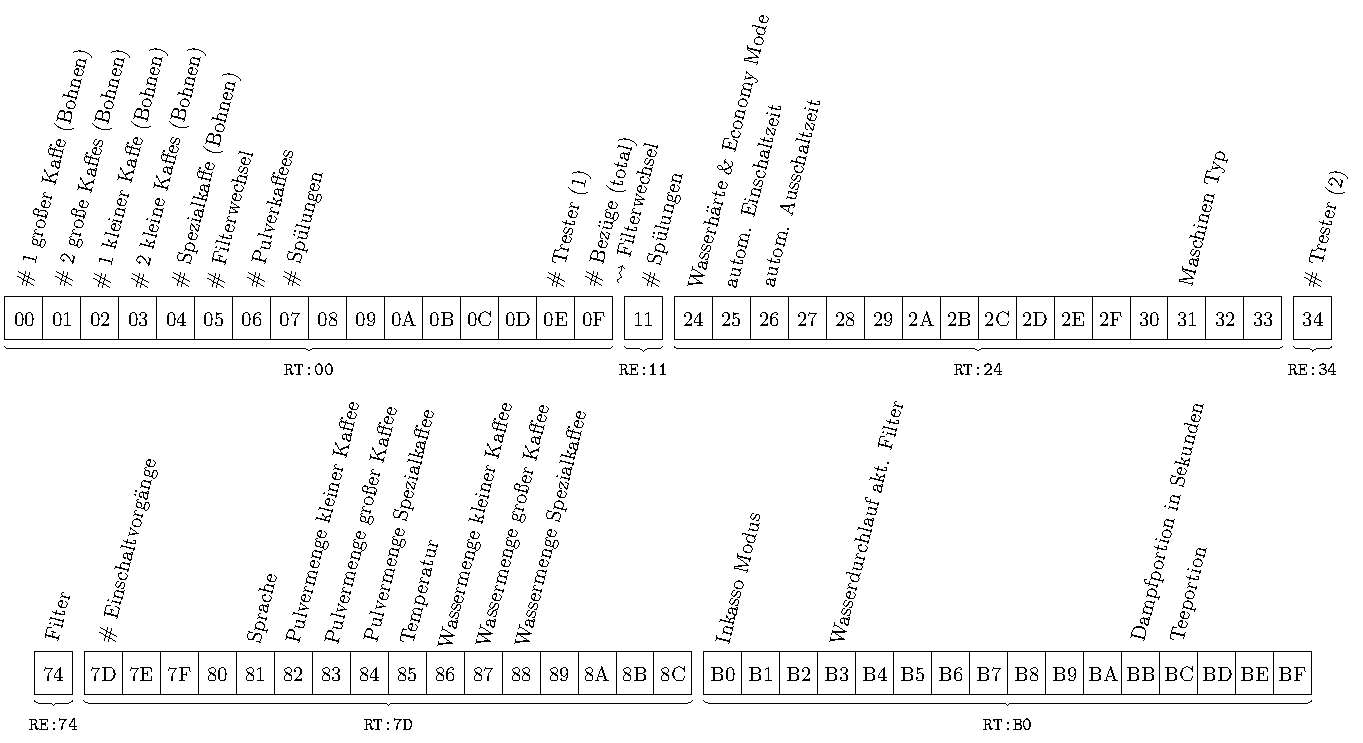
\includegraphics[scale=0.94]{images/chapter_5/API-EEPROM}
    \caption{Abgefragte Speicherstellen für die \ac{API} im \ac{EEPROM} (1 Kästchen $\equiv$ 1 Wort)}
    \label{fig:API-EEPROM}
  \end{center}
\end{sidewaysfigure}
\begin{sidewaysfigure}
  \begin{center}
    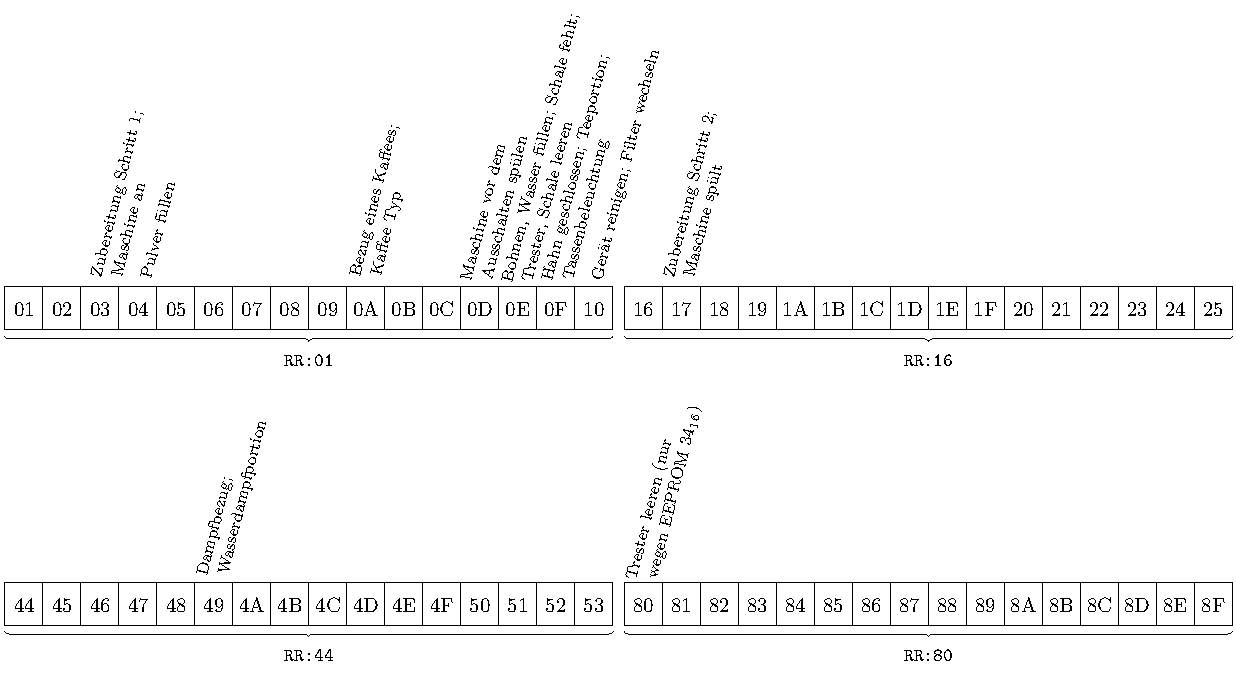
\includegraphics[scale=1]{images/chapter_5/API-RAM}
    \caption{Abgefragte Speicherstellen für die \ac{API} im \ac{RAM} (1 Kästchen $\equiv$ 1 Byte)}
    \label{fig:API-RAM}
  \end{center}
\end{sidewaysfigure}

\todo
Abgefragte Speicherstellen für die \ac{API} im \ac{EEPROM}: Abbildung~\ref{fig:API-EEPROM}

Abgefragte Speicherstellen für die \ac{API} im \ac{RAM}: Abbildung~\ref{fig:API-RAM}
\todo

\subsection{Display}\label{sec:Display}
Das Display der "`Jura Impressa S9"' umfasst zwei Zeilen mit je acht Zeichen, die wiederum mit je $5 \times 5$ Lichtpunkten dargestellt werden.
Tabelle~\ref{tbl:Displaysymbole} zeigt die verfügbaren Schriftzeichen auf.
Es handelt sich um arabische Zahlen, große lateinische Buchstaben sowie ein paar Sonderzeichen, die unter anderem eine Skala darstellen können.

$0_{10}$ bis $31_{10}$ und alle \ac{ASCII}-Zeichen über $97_{10}$, auch aus der erweiterten \ac{ASCII}-Tabelle von $128_{10}$ bis $255_{10}$ und darüber, stellt der Kaffeevollautomat nicht mehr als eindeutig bekannte \ac{ASCII}-Zeichen dar.
Es handelt sich höchstens um verpixeltes Kanji und wurde in der Tabelle ausgelassen.

\begin{tuhhtable}
  \newcommand{\display}[1]{\includegraphics[height=2ex]{images/chapter_5/display/#1.png}}
  \footnotesize\centering
  \begin{tabular}[tp]{rrcc   L{1mm}   rrcc}
%
  \THc{3}{c}{ASCII} & \THc{1}{c}{Kaffeevollautomat} &   \TRhc{1}{l}{}   &   \THc{3}{c}{ASCII} & \THc{1}{c}{Kaffeevollautomat} \\
  \THsub{1}{r}{hex} & \THsub{1}{r}{dez} & \THsub{1}{c}{Zeichen} & \THsub{1}{c}{Display} &   \TRhc{1}{l}{}   & \THsub{1}{r}{hex} & \THsub{1}{r}{dez} & \THsub{1}{c}{Zeichen} & \THsub{1}{c}{Display} \\
%
%  \abovebodyrule
%
       & {\tiny 0 – 31} & {\tiny$\ldots$} & {\tiny$\ldots$}   & \TRhc{1}{l}{} &   0x41 & 65            & A                          & A \\\TRc
  0x20 & 32             & Leerzeichen     & Leerzeichen       & \TRhc{1}{l}{} &   0x42 & 66            & B                          & B \\
  0x21 & 33             & !               & \_                & \TRhc{1}{l}{} &   0x43 & 67            & C                          & C \\\TRc
  0x22 & 34             & "               & \display{34}      & \TRhc{1}{l}{} &   0x44 & 68            & D                          & D \\
  0x23 & 35             & \#              & \display{35}      & \TRhc{1}{l}{} &   0x45 & 69            & E                          & E \\\TRc
  0x24 & 36             & \$              & \display{36}      & \TRhc{1}{l}{} &   0x46 & 70            & F                          & F \\
  0x25 & 37             & \%              & \display{37}      & \TRhc{1}{l}{} &   0x47 & 71            & G                          & G \\\TRc
  0x26 & 38             & \&              & \display{38}      & \TRhc{1}{l}{} &   0x48 & 72            & H                          & H \\
  0x27 & 39             & '               & \display{39}      & \TRhc{1}{l}{} &   0x49 & 73            & I                          & I \\\TRc
  0x28 & 40             & (               & \display{40}      & \TRhc{1}{l}{} &   0x4A & 74            & J                          & J \\
  0x29 & 41             & )               & \display{41}      & \TRhc{1}{l}{} &   0x4B & 75            & K                          & K \\\TRc
  0x2A & 42       & \textasteriskcentered & \display{42}      & \TRhc{1}{l}{} &   0x4C & 76            & L                          & L \\
  0x2B & 43             & +               & +                 & \TRhc{1}{l}{} &   0x4D & 77            & M                          & M \\\TRc
  0x2C & 44             & ,               & ,                 & \TRhc{1}{l}{} &   0x4E & 78            & N                          & N \\
  0x2D & 45             & -               & -                 & \TRhc{1}{l}{} &   0x4F & 79            & O                          & O \\\TRc
  0x2E & 46             & .               & .                 & \TRhc{1}{l}{} &   0x50 & 80            & P                          & P \\
  0x2F & 47             & /               & /                 & \TRhc{1}{l}{} &   0x51 & 81            & Q                          & Q \\\TRc
  0x30 & 48             & 0               & 0                 & \TRhc{1}{l}{} &   0x52 & 82            & R                          & R \\
  0x31 & 49             & 1               & 1                 & \TRhc{1}{l}{} &   0x53 & 83            & S                          & S \\\TRc
  0x32 & 50             & 2               & 2                 & \TRhc{1}{l}{} &   0x54 & 84            & T                          & T \\
  0x33 & 51             & 3               & 3                 & \TRhc{1}{l}{} &   0x55 & 85            & U                          & U \\\TRc
  0x34 & 52             & 4               & 4                 & \TRhc{1}{l}{} &   0x56 & 86            & V                          & V \\
  0x35 & 53             & 5               & 5                 & \TRhc{1}{l}{} &   0x57 & 87            & W                          & W \\\TRc
  0x36 & 54             & 6               & 6                 & \TRhc{1}{l}{} &   0x58 & 88            & X                          & X \\
  0x37 & 55             & 7               & 7                 & \TRhc{1}{l}{} &   0x59 & 89            & Y                          & Y \\\TRc
  0x38 & 56             & 8               & 8                 & \TRhc{1}{l}{} &   0x5A & 90            & Z                          & Z \\
  0x39 & 57             & 9               & 9                 & \TRhc{1}{l}{} &   0x5B & 91            & [                          & \display{91} \\\TRc
  0x3A & 58             & :               & :                 & \TRhc{1}{l}{} &   0x5C & 92            & \textbackslash             & \display{92} \\
  0x3B & 59             & ;               & ;                 & \TRhc{1}{l}{} &   0x5D & 93            & ]                          & \display{93} \\\TRc
  0x3C & 60             & <               & <                 & \TRhc{1}{l}{} &   0x5E & 94            & \^{}                       & \display{94} \\
  0x3D & 61             & =               & =                 & \TRhc{1}{l}{} &   0x5F & 95            & \_                         & \display{95} \\\TRc
  0x3E & 62             & >               & >                 & \TRhc{1}{l}{} &   0x60 & 96            & `                          & \display{96} \\
  0x3F & 63             & ?               & ?                 & \TRhc{1}{l}{} &        & {\tiny97-127} & {\tiny a-z \{ | \} $\sim$} & {\tiny$\ldots$} \\\TRc
  0x40 & 64             & @               & \display{64}      & \TRhc{1}{l}{} &        &               &                            &   \\
%
   \belowbodyrule
%
  \end{tabular}
  \caption{Verfügbarer Zeichensatz des Displays}
  \label{tbl:Displaysymbole}
\end{tuhhtable}
